\section{Results}\label{sec:results}

To demonstrate the effectiveness of modulo unrolling in the Chapel Cyclic and Block Cyclic distributions, we present our results. We have compiled a suite of seventeen parallel benchmarks shown in Figure \ref{benchmarks}. Each benchmark is written in Chapel and contains loops with affine array accesses that have been transformed to use zippered iteration by hand, as discussed in \ref{sec:array_slicing}. Our suite of benchmarks contains programs with single, double, and triple nested affine loops. Additionally, our benchmark suite contains programs operating on one, two, and three dimensional distributed arrays. Fourteen of the seventeen benchmarks are taken from the Polybench suite of benchmarks and translated from C to Chapel by hand. The stencil9 benchmark was taken from the Chapel source trunk directory. The remaining two benchmarks, pascal and folding, were written by our group. pascal is an additional benchmark other than jacobi1D that is able to test Block Cyclic with modulo unrolling. folding is the only benchmark in our suite that has strided affine array accesses. 

To evaluate improvements due to modulo unrolling, we run our benchmarks using Cyclic and Block Cyclic distributions from the 1.8.0 release of the Chapel compiler as well as Cyclic and Block Cylic distributions that have been modified to perform modulo unroling, as described in Sections \ref{sec:cyclic_modulo} and \ref{sec:block_cyclic_modulo}. We measure both runtime and message count for each benchmark. 

When evaluating modulo unrolling used with the Block Cyclic distribution, we could only run two benchmarks out of our suite of seventeen because of limitations within the distribution. Many of our benchmarks operate on two or three dimensional arrays and all require array slicing for the modulo unrolling optimization to apply. Both array slicing of multi-dimensional arrays and array slicing containing strides for one-dimensional arrays are not yet supported in the Block Cyclic distribution. Implementing such features reamined outside the scope of this work. There was no limitation when evaluating modulo unrolling with the Cyclic distribution, and all seventeen benchmarks were tested.

Figures \ref{cyclic_runtime} and \ref{cyclic_message_count} compare the normalized runtimes and message counts respectively for the Cyclic distribution and Cyclic distribution with modulo unrolling. For 8 of the 11 benchmarks, we see reductions in runtime when the modulo unrolling optimization is applied. On average, modulo unrolling results in a 45 percent decrease in runtime. For 9 of the 11 benchmarks, we see reductions in message counts when the modulo unrolling optimization is applied. On average, modulo unrolling results in 76 percent fewer messages. 

Figures \ref{block_cyclic_runtime} and \ref{block_cyclic_message_count} compare the normalized runtimes and message counts respectively for the Block Cyclic distribution and Block Cyclic distribution with modulo unrolling. For both benchmarks, we see reductions in runtime when the modulo unrolling optimization is applied. On average, modulo unrolling results in a 52 percent decrease in runtime. For both benchmarks, we see reductions in message counts when the modulo unrolling optimization is applied. On average, modulo unrolling results in 72 percent fewer messages. 


\begin{figure}
	\begin{center}
	\includegraphics[scale=0.60]{./Figures/Benchmarks.pdf}
	\caption{Benchmark suite. Benchmarks with $\dagger$ are taken from the Chapel Trunk test directory. Benchmarks with $\ddagger$ were developed on our own in order to test specific data access patterns. }
	\label{benchmarks}
	\end{center}
\end{figure}

\begin{figure}
	\begin{center}
	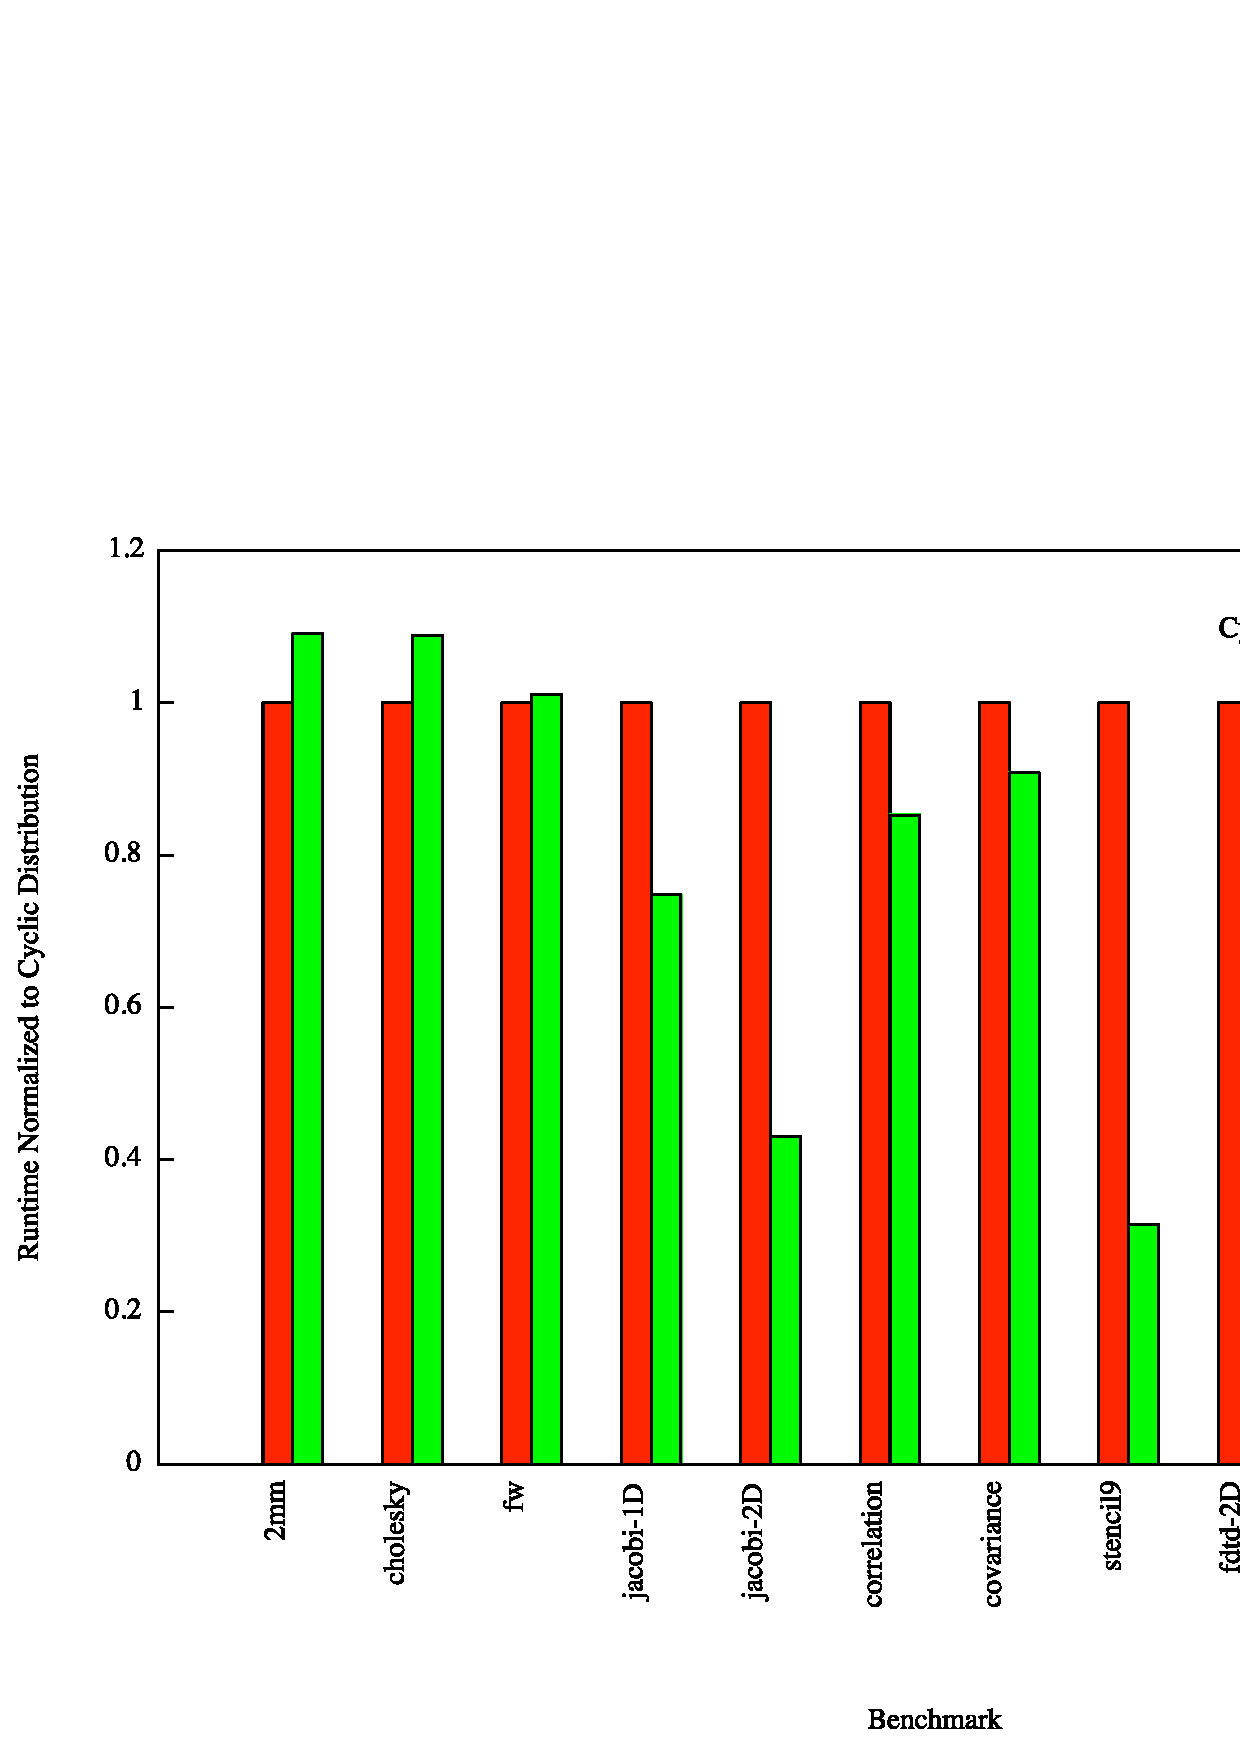
\includegraphics[scale=0.30]{./Figures/cyclic_runtime}
	\caption{Cyclic runtime.}
	\label{cyclic_runtime}
	\end{center}
\end{figure}

\begin{figure}
	\begin{center}
	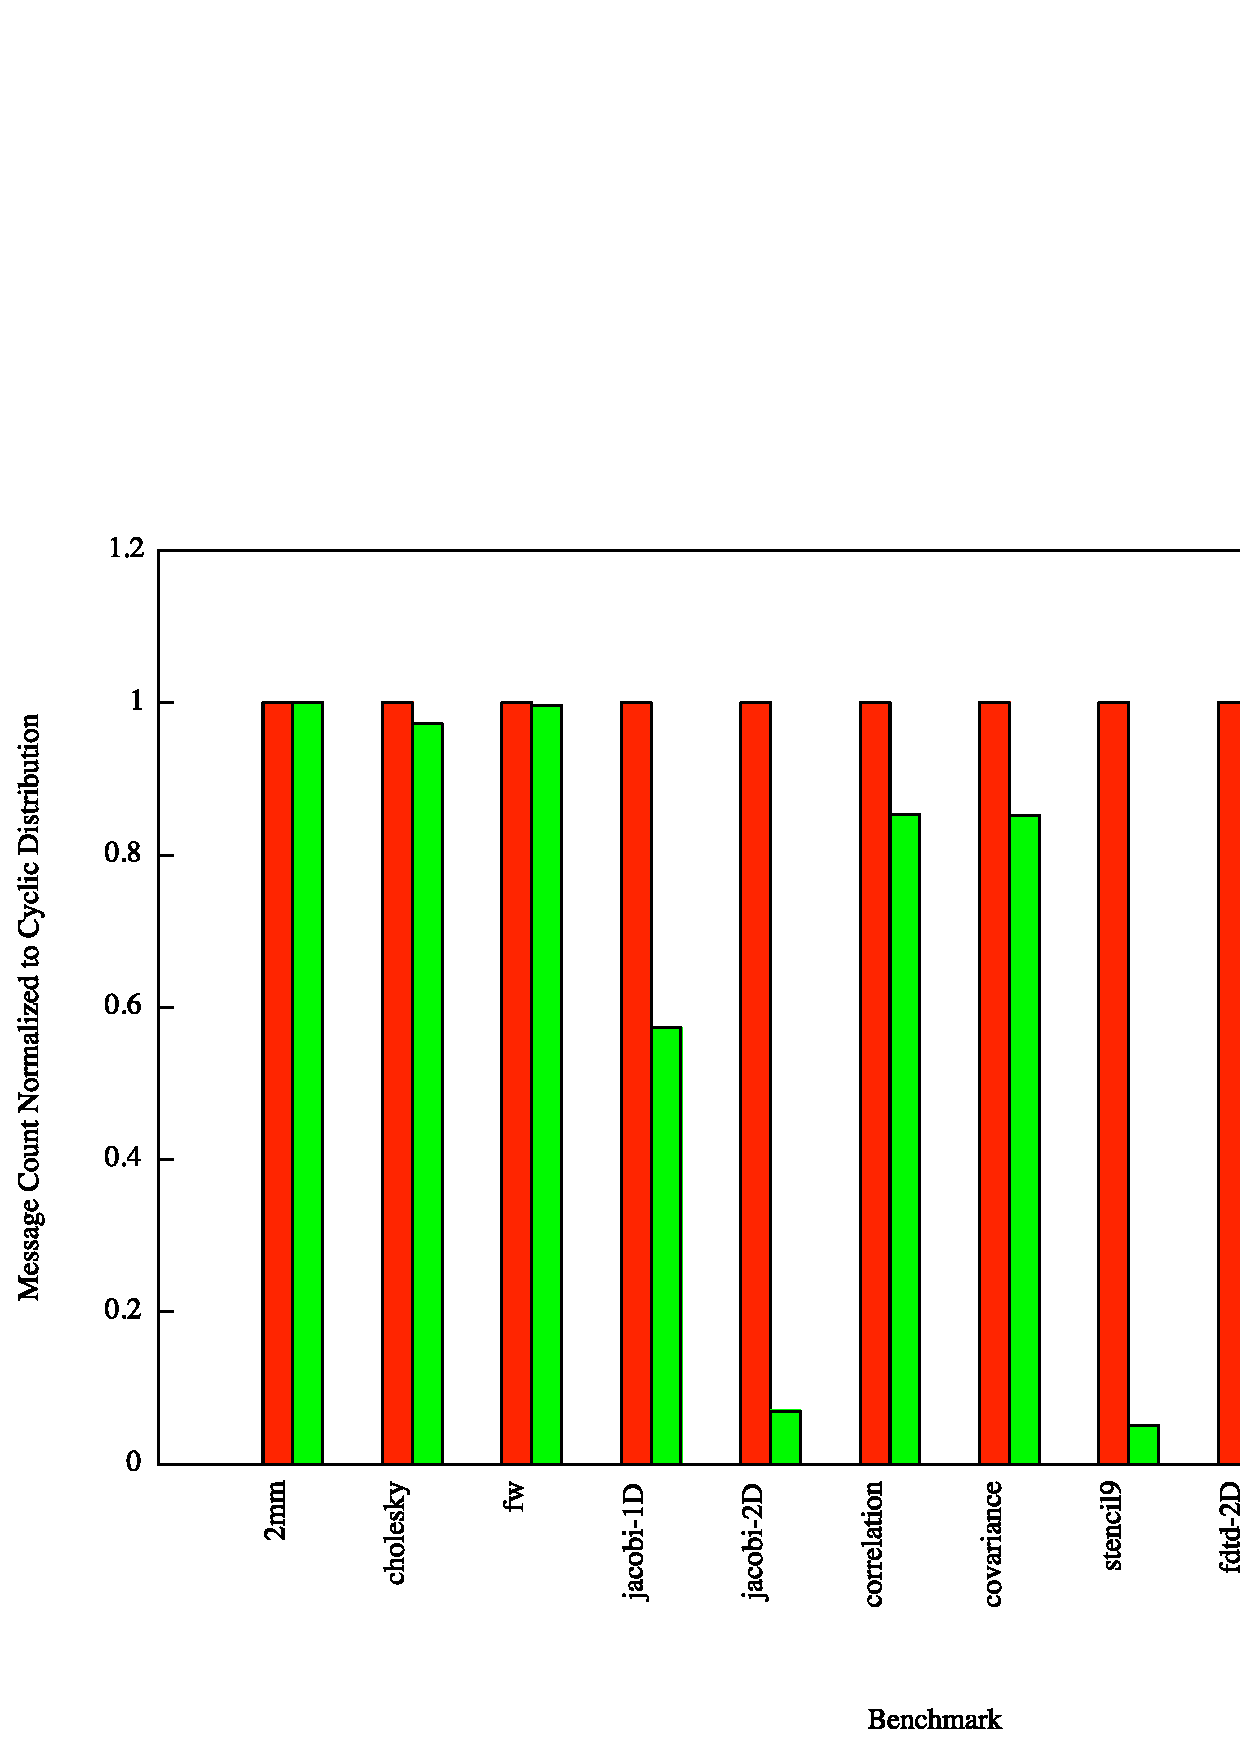
\includegraphics[scale=0.30]{./Figures/cyclic_message_count}
	\caption{Cyclic message count.}
	\label{cyclic_message_count}
	\end{center}
\end{figure}

\begin{figure}
	\begin{center}
	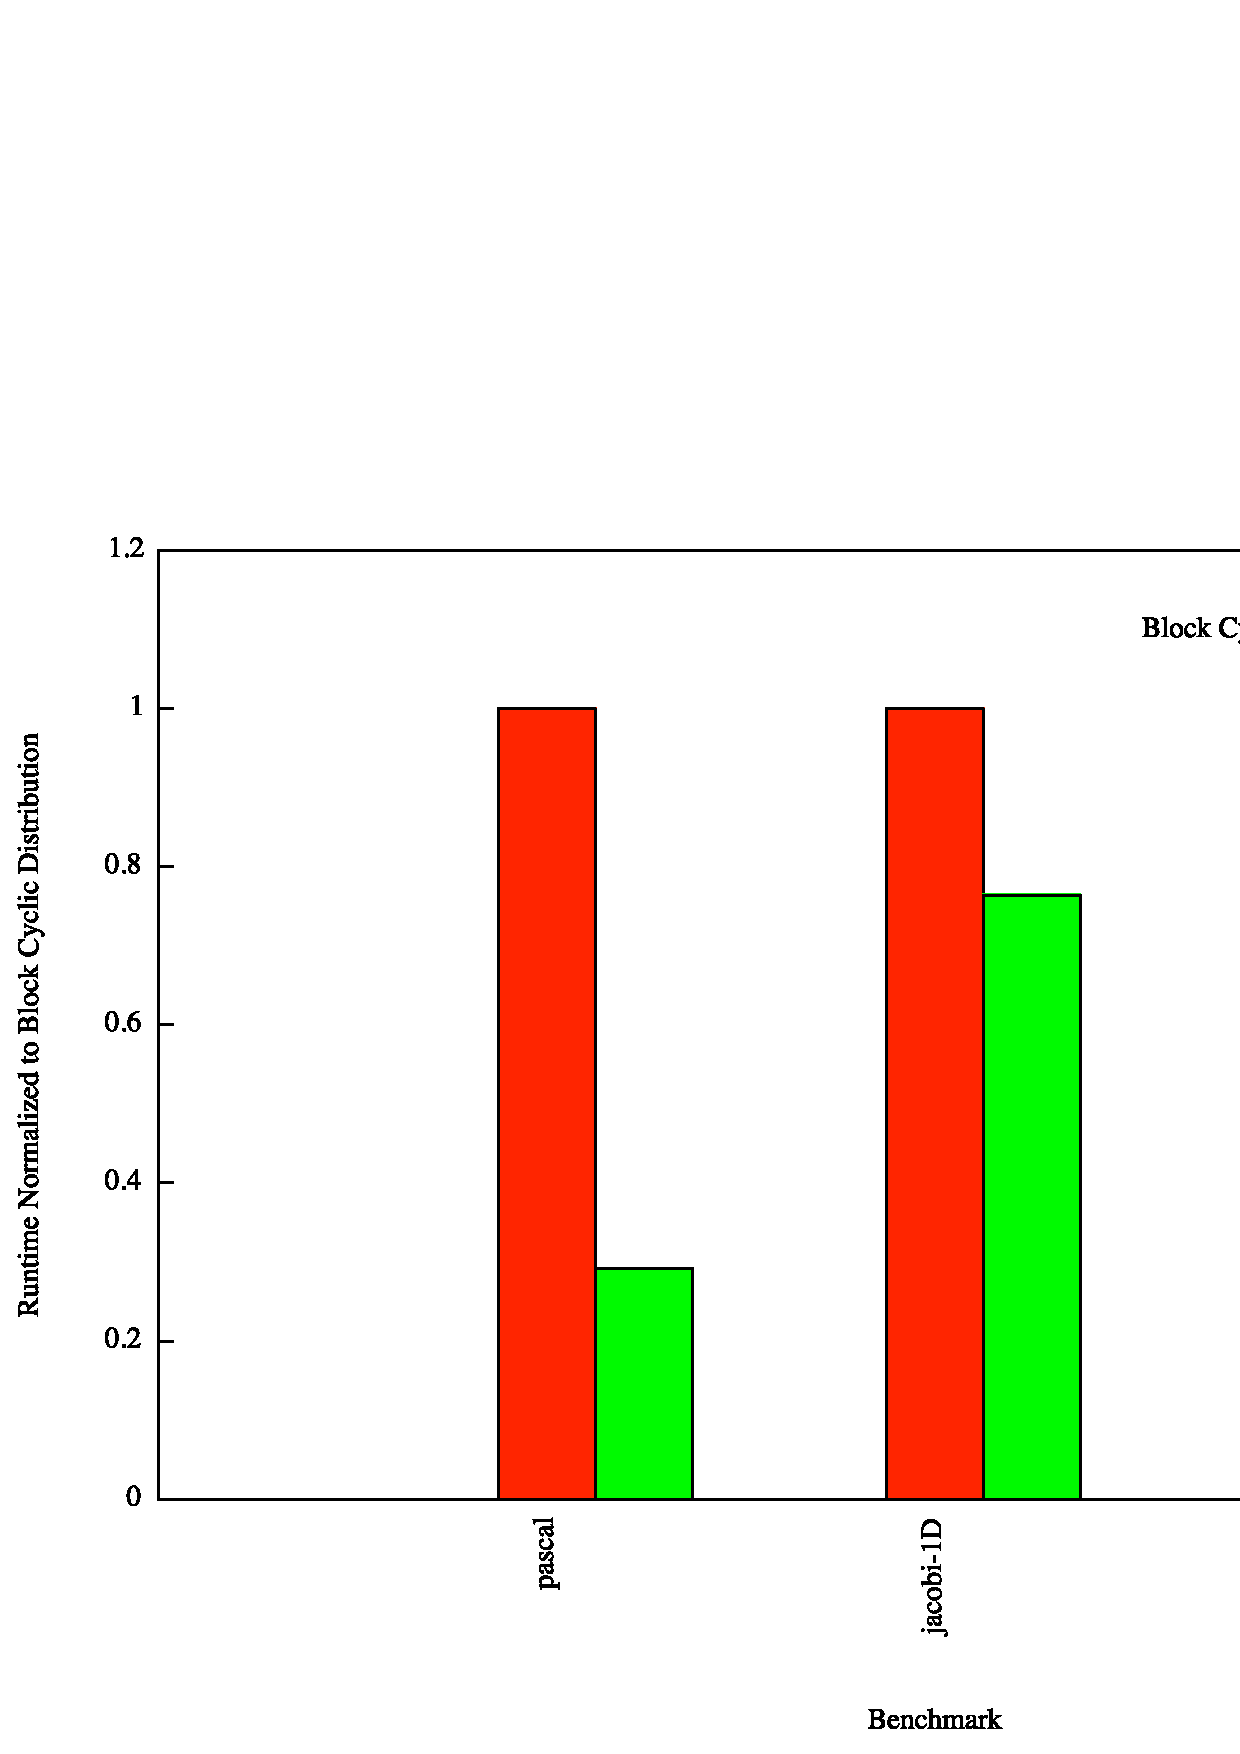
\includegraphics[scale=0.30]{./Figures/block_cyclic_runtime}
	\caption{Block Cyclic runtime.}
	\label{block_cyclic_runtime}
	\end{center}
\end{figure}

\begin{figure}
	\begin{center}
	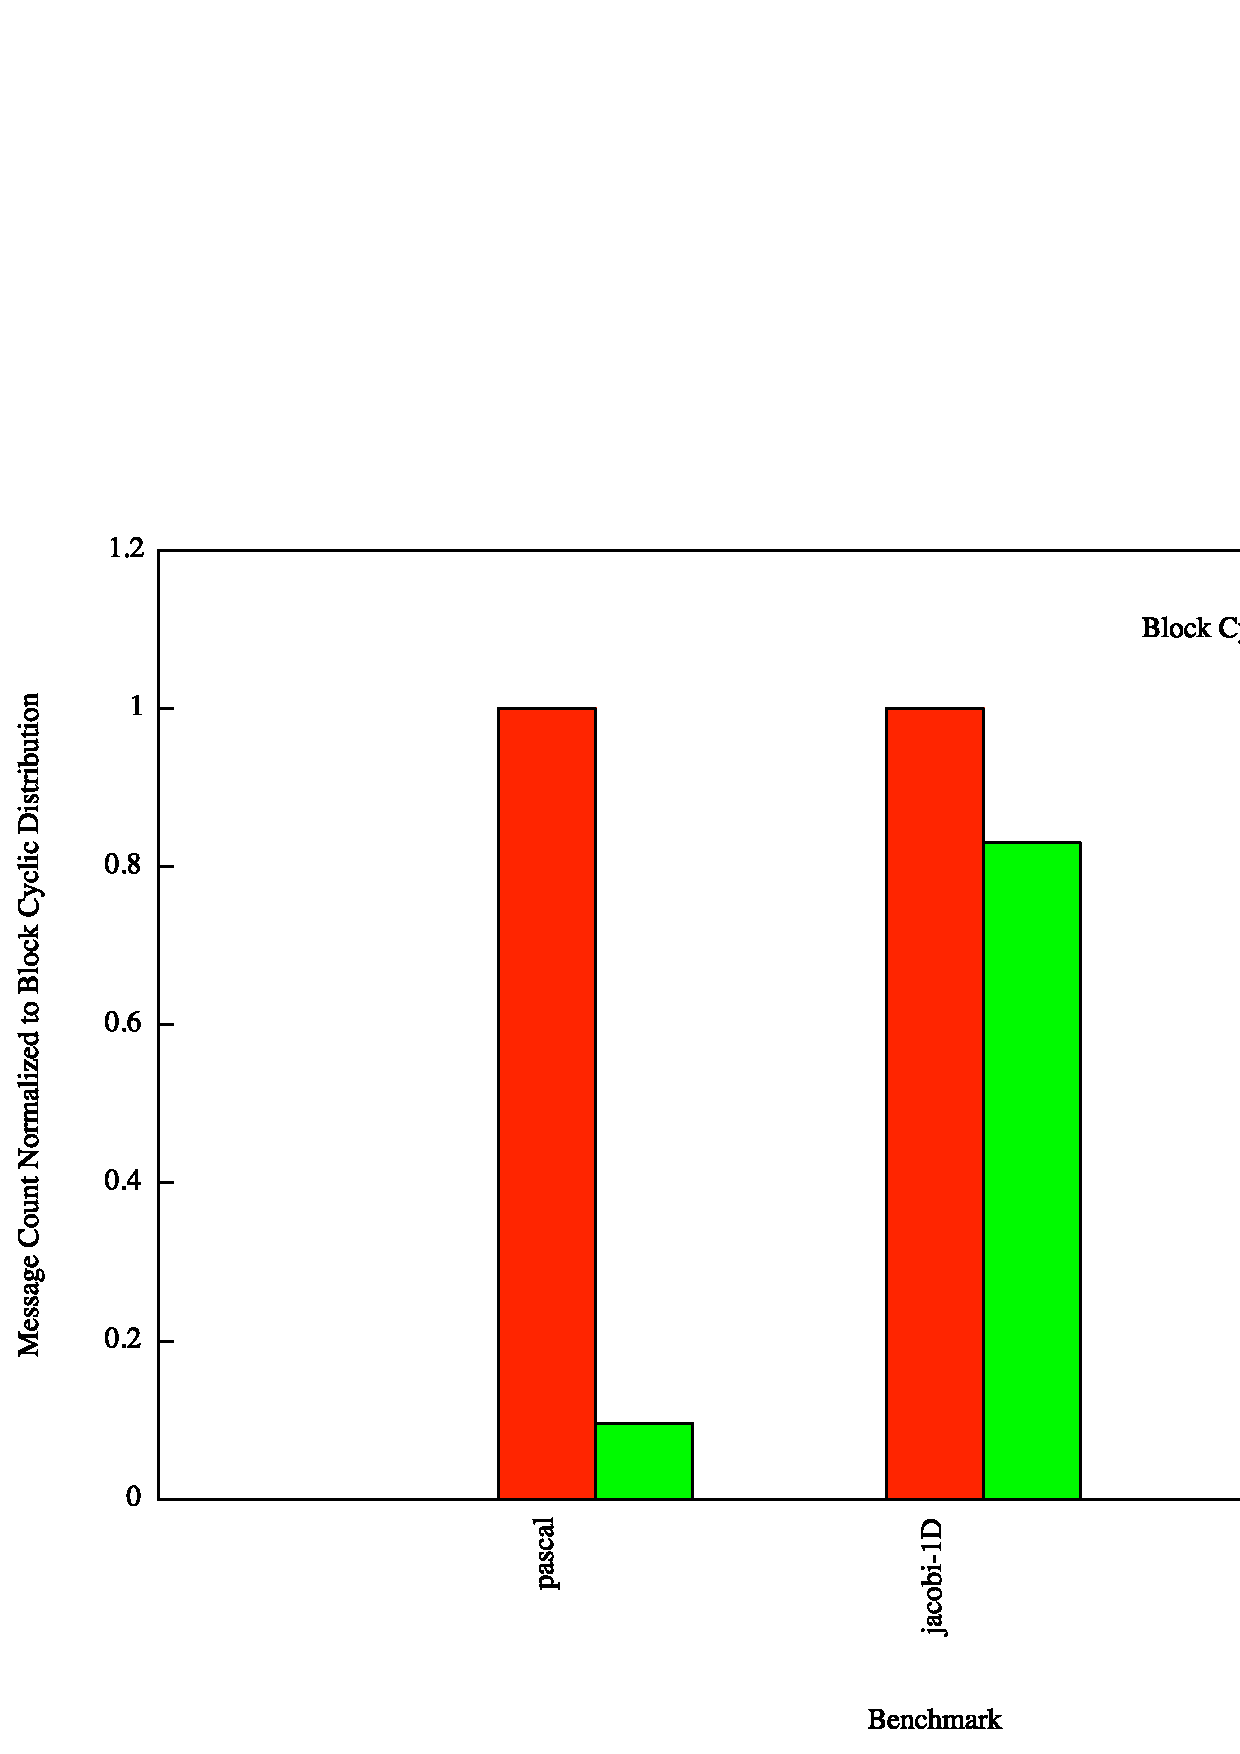
\includegraphics[scale=0.30]{./Figures/block_cyclic_message_count}
	\caption{Block Cyclic message count.}
	\label{block_cyclic_message_count}
	\end{center}
\end{figure}
